\begin{center}

  \begin{tabular}{rp{16cm}lp{20cm}}%{rl}

  % after \\: \hline or \cline{col1-col2} \cline{col3-col4} ...

  论文地址:& \href{https://papers.nips.cc/paper/2017/file/3f5ee243547dee91fbd053c1c4a845aa-Paper.pdf}{https://papers.nips.cc/paper/2017/file/3f5ee243547dee91fbd053c1c4a845aa-Paper.pdf} \\
  来源:& NIPS, 2017 \\
  作者:& Ashish Vaswani, et al. \\

  源码:& \href{https://github.com/tensorflow/tensor2tensor}{tensor2tensor} \\

%  slides:& \href{http://yunshengb.com/wp-content/uploads/2017/03/nips_2018_r2l_workshop_talk.pdf}{{\footnotesize Convolutional Set Matching for Graph Similarity}}\\

  关键词:& \textbf{Sequecnce Modeling, Neural Machine Translation} \\

  写于:& \date{2021-03-07}

  \end{tabular}

\end{center}

该论文\cite{vaswani2017attention}针对序列转换(Sequence Transduction)问题中常见的弊端,提出使用Attention来完成Sequence Transduction,提出了新的网络结构 --- Transformer。

\paragraph{问题定义}在Sequence Transduction领域中,通常是基于encoder-decoder形式的循环神经网络或CNN的。也存在一些模型使用注意力机制将encoder和decoder连接起来。该论文提出了一种完全基于注意力机制的新型网络 --- Transformer,不需要RNN或CNN。

在对序列进行处理时,RNN通常沿着输入/输出序列的顺序进行计算,将序列中元素的位置与计算的步骤相对齐。这样的处理方式看似天然地保留了序列形式,但是使得计算只能串行进行,难以并行,而且对于长序列的计算还会带来内存容量限制的问题。虽然目前已经有一些相关的工作关于RNN的并行化,但是RNN串行计算的问题依然存在。

注意力机制已经成为了序列建模中不可或缺的一部分,在建模序列中依赖的时候能够不用考虑输入/输出中的距离。但是之前的工作都是用于起连接作用,本文则将encoder-decoder完全建立在注意力机制上来完成序列的建模问题。并在机器翻译任务中检测了Transformer的效果。


\paragraph{Transformer}
\begin{figure}[h]
	\centering
	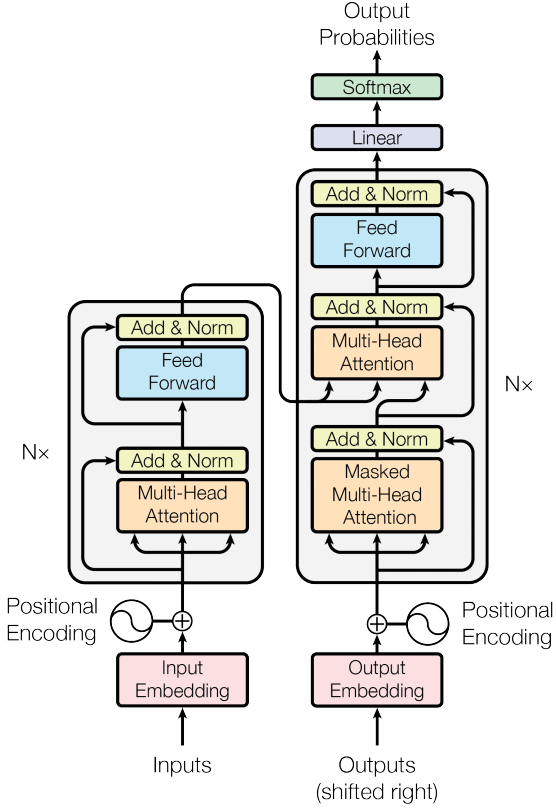
\includegraphics[width=.5\textwidth]{pics/Transformer.PNG}
	\caption{Transformer Architecture}
	\label{fig:transformer}
\end{figure}

\subparagraph{Encoder and Decoder}
Transformer的结构如Fig.\ref{fig:transformer}所示,其中左边为$N$个相同的layer堆叠起来的组成的encoder,右边为$N$个相同的layer堆叠起来组成的decoder。组成encoder的layer又两部分组成:Multi-head Attention、Fully connected Feed Forward。组成encoder的layer由三部分组成:两个Multi-head Attention、Fully connected Feed Forward。以上的Multi-head Attention和Fully connected FFN都有残差连接和layer normalization。这样每一部分的输出都可以表示为:$LayerNorm(x + Sublayer(x))$,其中$Sublayer$就是Multi-head Attention或Fully connected FFN。

其实Encoder和Decoder都是由Multi-head Attention和Fully connected FFN组成的,但是二者在Self-Attention上有一些差别。Decoder修改了Self-Attention,是为了保证\tbc{red}{在预测$i$处的输出时,只能依赖$i$之前的输出,同时也是为了保持自回归(auto-regressive)的性质}。

\subparagraph{Attention}
一个注意力函数可以描述为:将一个query与一系列的key-value对(pair)进行映射得到一个输出,其中的query、keys、values和输出均为向量。输出时values的加权求和,values对应的权是通过query与key计算得到的。

\begin{figure}[h]
	\centering
	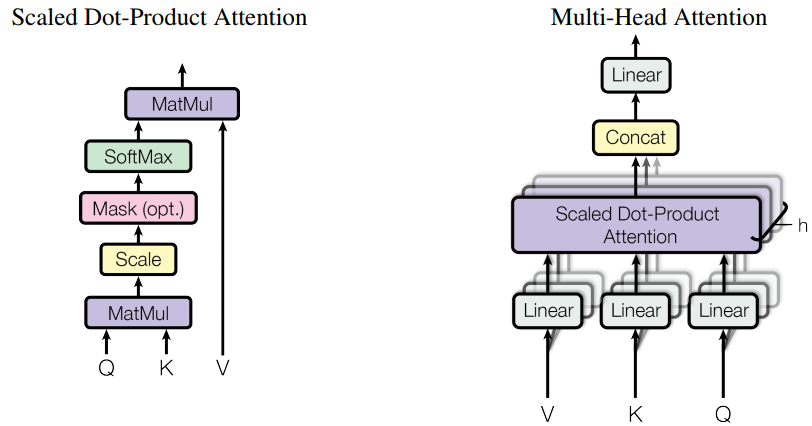
\includegraphics[width=.8\textwidth]{pics/Scaled Dot-Production Attention and Multi-Head Attention.PNG}
	\caption{Scaled Dot-Production Attention与Multi-Head Attention}
	\label{fig:scaled dot-product attention and multi-head attention}
\end{figure}

该论文中采用的是\textbf{Scaled Dot-Product Attention},其计算过程如Fig.\ref{fig:scaled dot-product attention and multi-head attention}所示,写成公式为:
$$
\operatorname{Attention}(Q, K, V)=\operatorname{softmax}\left(\frac{Q K^{T}}{\sqrt{d_{k}}}\right) V
$$
有两种常用的attention函数:additive attention和dot-product attention。该论文中使用的是dot-product attention,但是略微不同,是Scaled后的dot-product attention。\tbc{red}{为什么要对dot-product 进行scaled呢?}
\tbc{green}{当query、key的维度很大时,点积后的值可能会很大,可能会使softmax函数进入梯度很小的区域}。举个例子,加入q和k都是服从均值为0,方差为1的分布的随机变量,那么$q \cdot k = \sum_{i=1}^{d} q_i k_i$,结果的均值为0,但是方差为$d$。

论文中使用了\textbf{Multi-head Attention}。从Fig.\ref{fig:scaled dot-product attention and multi-head attention}可以看出,在进行Multi-head Attention之前,先对Q、K、V进行了线性映射:
$$
\begin{aligned}
	\operatorname{MultiHead}(Q, K, V) &=\text { Concat }\left(\text { head }_{1}, \ldots, \text { head }_{\mathrm{h}}\right) W^{O} \\
	\quad \text { where head }_{\mathrm{i}} &=\text { Attention }\left(Q W_{i}^{Q}, K W_{i}^{K}, V W_{i}^{V}\right)
\end{aligned}
$$

在Multi-Head Attention后就是\textbf{Position-wise Feed-Forward Networks}。从名字 --- Position-wise也可以看出,Multi-head Attention的输出是逐个通过FFN的。\tbc{red}{在输入Attention函数之前,各个位置上的元素可以看作是独立的,不包含元素之间的依赖关系,经过Attention函数后,各个元素不仅包含了本身的含义还包含了与其他元素的依赖关系。所以不需要串行地通过FFN,FFN这一步操作是可以并行化的}。

因为Transformer本身是不包含循环和卷积的,为了使模型利用序列中的顺序,论文中将\textbf{Positional Encoding}“加”到输入序列中的元素上。论文中使用的Positional-Encoding:
$$
\begin{aligned}
	P E_{(p o s, 2 i)} &=\sin \left(p o s / 10000^{2 i / d_{\text {model }}}\right) \\
	P E_{(p o s, 2 i+1)} &=\cos \left(p o s / 10000^{2 i / d_{\text {model }}}\right)
\end{aligned}
$$
其中$pos,i$分别表示position和位置编码的维度。作者选用这样的位置编码的原因:\tbc{red}{使不同位置的元素能够通过相对位置更好地与当前元素建立关系,因为对于任意固定的$k$,$PE_{pos+k}$可以表示为$PE_{pos}$的线性函数}。

\paragraph{Why Self-Attention}
$$
\begin{array}{lccc}
	\hline \text { Layer Type } & \text { Complexity per Layer } & \begin{array}{c}
		\text { Sequential } \\
		\text { Operations }
	\end{array} & \text { Maximum Path Length } \\
	\hline \text { Self-Attention } & O\left(n^{2} \cdot d\right) & O(1) & O(1) \\
	\text { Recurrent } & O\left(n \cdot d^{2}\right) & O(n) & O(n) \\
	\text { Convolutional } & O\left(k \cdot n \cdot d^{2}\right) & O(1) & O\left(\log _{k}(n)\right) \\
	\text { Self-Attention (restricted) } & O(r \cdot n \cdot d) & O(1) & O(n / r) \\
	\hline
	\label{rnn-cnn-attention}
\end{array}
$$
与RNN/CNN相比,使用Self-Attention主要有三个原因:
\begin{itemize}
	\item 计算复杂度
	\item 可并行的计算量
	\item 长范围依赖关系中的路径长度(注意:\textbf{长范围的依赖不一定代表距离远})。路径越短,越容易学习到长范围的依赖。Self-Attention中将每个位置的元素都直接与其他位置的元素相连。从Attention的输入和输出来看,CNN和Attention之间是有一定相似性的,如Fig.\ref{fig:cnn-attention-multi head}所示。Multi-head能够捕捉多种关系。在较长的输入序列下,可以选择restricted的self-attention,即每个位置只考虑周围固定数量的邻居
\end{itemize}
三者的比较见Tab.\ref{rnn-cnn-attention}
\begin{figure}[h]
	\centering
	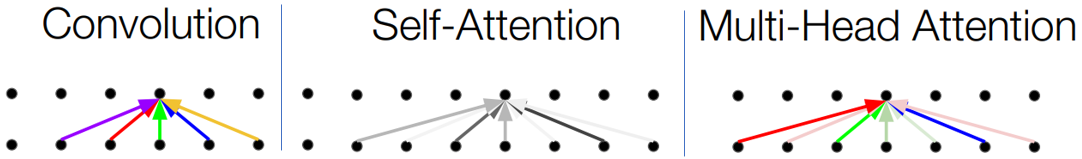
\includegraphics[width=.8\textwidth]{pics/CNN-Attention-Multi head.png}
	\caption{CNN、Attention、Multi-head Attention}
	\label{fig:cnn-attention-multi head}
\end{figure}

\paragraph{方法解决的问题/优势}

\begin{itemize}

	\item 提出了完全基于Attention机制的序列建模
	\item 基于Attention的Transformer中的大量操作都是可以并行的,大大降低计算的时间
	\item 对长范围依赖关系的建模

\end{itemize}



%\paragraph{方法的局限性/未来方向}

\begin{itemize}

	%\item 

\end{itemize}



\paragraph{Attention参考资料}
\begin{itemize}
	\item \href{http://nlp.seas.harvard.edu/2018/04/03/attention.html}{The Annotated Transformer --- Harvard Transformer tutorial}
	\item \href{https://jalammar.github.io/visualizing-neural-machine-translation-mechanics-of-seq2seq-models-with-attention/}{Visualizing A Neural Machine Translation Model (Mechanics of Seq2seq Models With Attention)}
	\item \href{https://jalammar.github.io/illustrated-transformer/}{The Illustrated Transformer}
\end{itemize}



